
%% bare_jrnl.tex
%% V1.4b
%% 2015/08/26
%% by Michael Shell
%% see http://www.michaelshell.org/
%% for current contact information.B8-85-84-AF-15-1B
%%
%% This is a skeleton file demonstrating the use of IEEEtran.cls
%% (requires IEEEtran.cls version 1.8b or later) with an IEEE
%% journal paper.
%%
%% Support sites: %% http://www.michaelshell.org/tex/ieeetran/
%% http://www.ctan.org/pkg/ieeetran
%% and
%% http://www.ieee.org/

%%*************************************************************************
%% Legal Notice:
%% This code is offered as-is without any warranty either expressed or
%% implied; without even the implied warranty of MERCHANTABILITY or
%% FITNESS FOR A PARTICULAR PURPOSE!
%% User assumes all risk.
%% In no event shall the IEEE or any contributor to this code be liable for
%% any damages or losses, including, but not limited to, incidental,
%% consequential, or any other damages, resulting from the use or misuse
%% of any information contained here.
%%
%% All comments are the opinions of their respective authors and are not
%% necessarily endorsed by the IEEE.
%%
%% This work is distributed under the LaTeX Project Public License (LPPL)
%% ( http://www.latex-project.org/ ) version 1.3, and may be freely used,
%% distributed and modified. A copy of the LPPL, version 1.3, is included
%% in the base LaTeX documentation of all distributions of LaTeX released
%% 2003/12/01 or later.
%% Retain all contribution notices and credits.
%% ** Modified files should be clearly indicated as such, including  **
%% ** renaming them and changing author support contact information. **
%%*************************************************************************


% *** Authors should verify (and, if needed, correct) their LaTeX system  ***
% *** with the testflow diagnostic prior to trusting their LaTeX platform ***
% *** with production work. The IEEE's font choices and paper sizes can   ***
% *** trigger bugs that do not appear when using other class files.       ***                          ***
% The testflow support page is at:
% http://www.michaelshell.org/tex/testflow/



\documentclass[journal]{IEEEtran}
%
% If IEEEtran.cls has not been installed into the LaTeX system files,
% manually specify the path to it like:
% \documentclass[journal]{../sty/IEEEtran}





% Some very useful LaTeX packages include:
% (uncomment the ones you want to load)


% *** MISC UTILITY PACKAGES ***
%
%\usepackage{ifpdf}
% Heiko Oberdiek's ifpdf.sty is very useful if you need conditional
% compilation based on whether the output is pdf or dvi.
% usage:
% \ifpdf
%   % pdf code
% \else
%   % dvi code
% \fi
% The latest version of ifpdf.sty can be obtained from:
% http://www.ctan.org/pkg/ifpdf
% Also, note that IEEEtran.cls V1.7 and later provides a builtin
% \ifCLASSINFOpdf conditional that works the same way.
% When switching from latex to pdflatex and vice-versa, the compiler may
% have to be run twice to clear warning/error messages.






% *** CITATION PACKAGES ***
%
%\usepackage{cite}
% cite.sty was written by Donald Arseneau
% V1.6 and later of IEEEtran pre-defines the format of the cite.sty package
% \cite{} output to follow that of the IEEE. Loading the cite package will
% result in citation numbers being automatically sorted and properly
% "compressed/ranged". e.g., [1], [9], [2], [7], [5], [6] without using
% cite.sty will become [1], [2], [5]--[7], [9] using cite.sty. cite.sty's
% \cite will automatically add leading space, if needed. Use cite.sty's
% noadjust option (cite.sty V3.8 and later) if you want to turn this off
% such as if a citation ever needs to be enclosed in parenthesis.
% cite.sty is already installed on most LaTeX systems. Be sure and use
% version 5.0 (2009-03-20) and later if using hyperref.sty.
% The latest version can be obtained at:
% http://www.ctan.org/pkg/cite
% The documentation is contained in the cite.sty file itself.






% *** GRAPHICS RELATED PACKAGES ***
%
\ifCLASSINFOpdf
  % \usepackage[pdftex]{graphicx}
  % declare the path(s) where your graphic files are
  % \graphicspath{{../pdf/}{../jpeg/}}
  % and their extensions so you won't have to specify these with
  % every instance of \includegraphics
  % \DeclareGraphicsExtensions{.pdf,.jpeg,.png}
\else
  % or other class option (dvipsone, dvipdf, if not using dvips). graphicx
  % will default to the driver specified in the system graphics.cfg if no
  % driver is specified.
  % \usepackage[dvips]{graphicx}
  % declare the path(s) where your graphic files are
  % \graphicspath{{../eps/}}
  % and their extensions so you won't have to specify these with
  % every instance of \includegraphics
  % \DeclareGraphicsExtensions{.eps}
\fi
% graphicx was written by David Carlisle and Sebastian Rahtz. It is
% required if you want graphics, photos, etc. graphicx.sty is already
% installed on most LaTeX systems. The latest version and documentation
% can be obtained at:
% http://www.ctan.org/pkg/graphicx
% Another good source of documentation is "Using Imported Graphics in
% LaTeX2e" by Keith Reckdahl which can be found at:
% http://www.ctan.org/pkg/epslatex
%
% latex, and pdflatex in dvi mode, support graphics in encapsulated
% postscript (.eps) format. pdflatex in pdf mode supports graphics
% in .pdf, .jpeg, .png and .mps (metapost) formats. Users should ensure
% that all non-photo figures use a vector format (.eps, .pdf, .mps) and
% not a bitmapped formats (.jpeg, .png). The IEEE frowns on bitmapped formats
% which can result in "jaggedy"/blurry rendering of lines and letters as
% well as large increases in file sizes.
%
% You can find documentation about the pdfTeX application at:
% http://www.tug.org/applications/pdftex


\usepackage{color}
\usepackage{amsmath}
\usepackage{amssymb}
\usepackage{tabularx}

\usepackage{epsfig}
%\usepackage[colorlinks=false, urlcolor=black, pdfborder={0 0 0}]{hyperref}
%\let\url\nolinkurl
%\usepackage[options]{nohyperref}  % This makes hyperref commands do nothing without errors
\usepackage{url}  % This makes \url work

%\usepackage[dvips]{epsfig}
\usepackage{etoolbox}
\apptocmd{\sloppy}{\hbadness 10000\relax}{}{}

\usepackage{longtable}
\usepackage{graphicx}
\usepackage[T1]{fontenc}
\usepackage{paralist}
\usepackage{enumitem}
%%%%%%%%%%%%for
\usepackage{adjustbox}
\usepackage{array}
\usepackage{booktabs}
\newcolumntype{C}{>{\centering\arraybackslash}X} % centered version of "X" type
\setlength{\extrarowheight}{1pt}
%\usepackage{lipsum}
\usepackage{multirow}

\newcolumntype{R}[2]{%
    >{\adjustbox{angle=#1,lap=\width-(#2)}\bgroup}%
    l%
    <{\egroup}%
}
\newcommand*\rot{\multicolumn{1}{R{90}{1em}}}% no optional argument here, please!

\usepackage{epstopdf}


\def\BibTeX{{\rm B\kern-.05em{\sc i\kern-.025em b}\kern-.08em
    T\kern-.1667em\lower.7ex\hbox{E}\kern-.125emX}}

\usepackage{pdflscape}
%\usepackage{subfigure}
\usepackage{tabularx}
\usepackage{xtab}
%\usepackage{supertabular}

\usepackage{booktabs, threeparttable}
\usepackage{array}
\newcolumntype{L}[1]{>{\raggedright\arraybackslash}p{#1}}

% *** MATH PACKAGES ***
\usepackage{algorithm}
\usepackage[noend]{algpseudocode}

\makeatletter
\def\BState{\State\hskip-\ALG@thistlm}
\makeatother

\algnewcommand\algorithmicswitch{\textbf{switch}}
\algnewcommand\algorithmiccase{\textbf{case}}
\algnewcommand\algorithmicassert{\texttt{assert}}
\algnewcommand\Assert[1]{\State \algorithmicassert(#1)}%
% New "environments"
\algdef{SE}[SWITCH]{Switch}{EndSwitch}[1]{\algorithmicswitch\ #1\ \algorithmicdo}{\algorithmicend\ \algorithmicswitch}%
\algdef{SE}[CASE]{Case}{EndCase}[1]{\algorithmiccase\ #1}{\algorithmicend\ \algorithmiccase}%
\algtext*{EndSwitch}%
\algtext*{EndCase}%





% *** SPECIALIZED LIST PACKAGES ***
%
%\usepackage{algorithmic}
% algorithmic.sty was written by Peter Williams and Rogerio Brito.
% This package provides an algorithmic environment fo describing algorithms.
% You can use the algorithmic environment in-text or within a figure
% environment to provide for a floating algorithm. Do NOT use the algorithm
% floating environment provided by algorithm.sty (by the same authors) or
% algorithm2e.sty (by Christophe Fiorio) as the IEEE does not use dedicated
% algorithm float types and packages that provide these will not provide
% correct IEEE style captions. The latest version and documentation of
% algorithmic.sty can be obtained at:
% http://www.ctan.org/pkg/algorithms
% Also of interest may be the (relatively newer and more customizable)
% algorithmicx.sty package by Szasz Janos:
% http://www.ctan.org/pkg/algorithmicx




% *** ALIGNMENT PACKAGES ***
%
%\usepackage{array}
% Frank Mittelbach's and David Carlisle's array.sty patches and improves
% the standard LaTeX2e array and tabular environments to provide better
% appearance and additional user controls. As the default LaTeX2e table
% generation code is lacking to the point of almost being broken with
% respect to the quality of the end results, all users are strongly
% advised to use an enhanced (at the very least that provided by array.sty)
% set of table tools. array.sty is already installed on most systems. The
% latest version and documentation can be obtained at:
% http://www.ctan.org/pkg/array


% IEEEtran contains the IEEEeqnarray family of commands that can be used to
% generate multiline equations as well as matrices, tables, etc., of high
% quality.




% *** SUBFIGURE PACKAGES ***
%\ifCLASSOPTIONcompsoc
%  \usepackage[caption=false,font=normalsize,labelfont=sf,textfont=sf]{subfig}
%\else
%  \usepackage[caption=false,font=footnotesize]{subfig}
%\fi
% subfig.sty, written by Steven Douglas Cochran, is the modern replacement
% for subfigure.sty, the latter of which is no longer maintained and is
% incompatible with some LaTeX packages including fixltx2e. However,
% subfig.sty requires and automatically loads Axel Sommerfeldt's caption.sty
% which will override IEEEtran.cls' handling of captions and this will result
% in non-IEEE style figure/table captions. To prevent this problem, be sure
% and invoke subfig.sty's "caption=false" package option (available since
% subfig.sty version 1.3, 2005/06/28) as this is will preserve IEEEtran.cls
% handling of captions.
% Note that the Computer Society format requires a larger sans serif font
% than the serif footnote size font used in traditional IEEE formatting
% and thus the need to invoke different subfig.sty package options depending
% on whether compsoc mode has been enabled.
%
% The latest version and documentation of subfig.sty can be obtained at:
% http://www.ctan.org/pkg/subfig




% *** FLOAT PACKAGES ***
%
%\usepackage{fixltx2e}
% fixltx2e, the successor to the earlier fix2col.sty, was written by
% Frank Mittelbach and David Carlisle. This package corrects a few problems
% in the LaTeX2e kernel, the most notable of which is that in current
% LaTeX2e releases, the ordering of single and double column floats is not
% guaranteed to be preserved. Thus, an unpatched LaTeX2e can allow a
% single column figure to be placed prior to an earlier double column
% figure.
% Be aware that LaTeX2e kernels dated 2015 and later have fixltx2e.sty's
% corrections already built into the system in which case a warning will
% be issued if an attempt is made to load fixltx2e.sty as it is no longer
% needed.
% The latest version and documentation can be found at:
% http://www.ctan.org/pkg/fixltx2e


%\usepackage{stfloats}
% stfloats.sty was written by Sigitas Tolusis. This package gives LaTeX2e
% the ability to do double column floats at the bottom of the page as well
% as the top. (e.g., "\begin{figure*}[!b]" is not normally possible in
% LaTeX2e). It also provides a command:
%\fnbelowfloat
% to enable the placement of footnotes below bottom floats (the standard
% LaTeX2e kernel puts them above bottom floats). This is an invasive package
% which rewrites many portions of the LaTeX2e float routines. It may not work
% with other packages that modify the LaTeX2e float routines. The latest
% version and documentation can be obtained at:
% http://www.ctan.org/pkg/stfloats
% Do not use the stfloats baselinefloat ability as the IEEE does not allow
% \baselineskip to stretch. Authors submitting work to the IEEE should note
% that the IEEE rarely uses double column equations and that authors should try
% to avoid such use. Do not be tempted to use the cuted.sty or midfloat.sty
% packages (also by Sigitas Tolusis) as the IEEE does not format its papers in
% such ways.
% Do not attempt to use stfloats with fixltx2e as they are incompatible.
% Instead, use Morten Hogholm'a dblfloatfix which combines the features
% of both fixltx2e and stfloats:
%
% \usepackage{dblfloatfix}
% The latest version can be found at:
% http://www.ctan.org/pkg/dblfloatfix




%\ifCLASSOPTIONcaptionsoff
%  \usepackage[nomarkers]{endfloat}
% \let\MYoriglatexcaption\caption
% \renewcommand{\caption}[2][\relax]{\MYoriglatexcaption[#2]{#2}}
%\fi
% endfloat.sty was written by James Darrell McCauley, Jeff Goldberg and
% Axel Sommerfeldt. This package may be useful when used in conjunction with
% IEEEtran.cls'  captionsoff option. Some IEEE journals/societies require that
% submissions have lists of figures/tables at the end of the paper and that
% figures/tables without any captions are placed on a page by themselves at
% the end of the document. If needed, the draftcls IEEEtran class option or
% \CLASSINPUTbaselinestretch interface can be used to increase the line
% spacing as well. Be sure and use the nomarkers option of endfloat to
% prevent endfloat from "marking" where the figures would have been placed
% in the text. The two hack lines of code above are a slight modification of
% that suggested by in the endfloat docs (section 8.4.1) to ensure that
% the full captions always appear in the list of figures/tables - even if
% the user used the short optional argument of \caption[]{}.
% IEEE papers do not typically make use of \caption[]'s optional argument,
% so this should not be an issue. A similar trick can be used to disable
% captions of packages such as subfig.sty that lack options to turn off
% the subcaptions:
% For subfig.sty:
% \let\MYorigsubfloat\subfloat
% \renewcommand{\subfloat}[2][\relax]{\MYorigsubfloat[]{#2}}
% However, the above trick will not work if both optional arguments of
% the \subfloat command are used. Furthermore, there needs to be a
% description of each subfigure *somewhere* and endfloat does not add
% subfigure captions to its list of figures. Thus, the best approach is to
% avoid the use of subfigure captions (many IEEE journals avoid them anyway)
% and instead reference/explain all the subfigures within the main caption.
% The latest version of endfloat.sty and its documentation can obtained at:
% http://www.ctan.org/pkg/endfloat
%
% The IEEEtran \ifCLASSOPTIONcaptionsoff conditional can also be used
% later in the document, say, to conditionally put the References on a
% page by themselves.




% *** PDF, URL AND HYPERLINK PACKAGES ***
%
%\usepackage{url}
% url.sty was written by Donald Arseneau. It provides better support for
% handling and breaking URLs. url.sty is already installed on most LaTeX
% systems. The latest version and documentation can be obtained at:
% http://www.ctan.org/pkg/url
% Basically, \url{my_url_here}.




% *** Do not adjust lengths that control margins, column widths, etc. ***
% *** Do not use packages that alter fonts (such as pslatex).         ***
% There should be no need to do such things with IEEEtran.cls V1.6 and later.
% (Unless specifically asked to do so by the journal or conference you plan
% to submit to, of course. )


% correct bad hyphenation here
%\hyphenation{op-tical net-works semi-conduc-tor}


\begin{document}
%
% paper title
% Titles are generally capitalized except for words such as a, an, and, as,
% at, but, by, for, in, nor, of, on, or, the, to and up, which are usually
% not capitalized unless they are the first or last word of the title.
% Linebreaks \\ can be used within to get better formatting as desired.
% Do not put math or special symbols in the title.
\title{Decentralised Reinforcement Learning in Fog-based Internet-of-Things}
%
%
% author names and IEEE memberships
% note positions of commas and nonbreaking spaces ( ~ ) LaTeX will not break
% a structure at a ~ so this keeps an author's name from being broken across
% two lines.
% use \thanks{} to gain access to the first footnote area
% a separate \thanks must be used for each paragraph as LaTeX2e's \thanks
% was not built to handle multiple paragraphs
%

\author{XXX~YYYY,
        and~ XXX~ZZZZ% <-this % stops a space
%\thanks{B. Omoniwa is with National Mathematical Centre, PMB 118, Abuja-Nigeria, email: tunjiomoniwa@gmail.com.}% <-this % stops a space

\thanks{Manuscript received March 14, 2019; revised July X, 2019.}
\thanks{Copyright (c) 2012 IEEE. Personal use of this material is permitted. However, permission to use this material for any other purposes must be obtained from the IEEE by sending a request to pubs-permissions@ieee.org.}
}

% note the % following the last \IEEEmembership and also \thanks -
% these prevent an unwanted space from occurring between the last author name
% and the end of the author line. i.e., if you had this:
%
% \author{....lastname \thanks{...} \thanks{...} }
%                     ^------------^------------^----Do not want these spaces!
%
% a space would be appended to the last name and could cause every name on that
% line to be shifted left slightly. This is one of those "LaTeX things". For
% instance, "\textbf{A} \textbf{B}" will typeset as "A B" not "AB". To get
% "AB" then you have to do: "\textbf{A}\textbf{B}"
% \thanks is no different in this regard, so shield the last } of each \thanks
% that ends a line with a % and do not let a space in before the next \thanks.
% Spaces after \IEEEmembership other than the last one are OK (and needed) as
% you are supposed to have spaces between the names. For what it is worth,
% this is a minor point as most people would not even notice if the said evil
% space somehow managed to creep in.



% The paper headers
\markboth{IEEE Internet of Things Journal,~Vol.~X, No.~X, August~2019}%
{YYYY \MakeLowercase{\textit{et al.}}: Decentralised Reinforcement Learning in Fog-based Internet-of-Things}
% The only time the second header will appear is for the odd numbered pages
% after the title page when using the twoside option.
%
% *** Note that you probably will NOT want to include the author's ***
% *** name in the headers of peer review papers.                   ***
% You can use \ifCLASSOPTIONpeerreview for conditional compilation here if
% you desire.




% If you want to put a publisher's ID mark on the page you can do it like
% this:
%\IEEEpubid{0000--0000/00\$00.00~\copyright~2015 IEEE}
% Remember, if you use this you must call \IEEEpubidadjcol in the second
% column for its text to clear the IEEEpubid mark.



% use for special paper notices
%\IEEEspecialpapernotice{(Invited Paper)}



% make the title area
\maketitle

% As a general rule, do not put math, special symbols or citations
% in the abstract or keywords.
\begin{abstract}
Reinforcement learning (RL) algorithms offers more insights about the overall futuristic functionalities for intelligent Internet-of-Things (IoT) devices. With the explosive growth in the number of IoT devices, as well as the highly-distributed deployments of these devices today, managing the IoT devices centrally becomes infeasible. As such, several disruptive paradigms have emerged, one of which is the fog computing-based IoT, which aim towards shifting computation, control, and decision-making closer to the network edge. However, mobility and power-constrain of these fog devices remains an issue of concern. In this paper, we apply a q-learning algorithm to minimize the outage in communication within a fog-based IoT network, by optimizing the power-control parameter of the agent, as well as optimizing the physical position. Furthermore, the agent was able to efficiently minimize the energy consumed by the fog relay and the IoT sensor, while guaranteeing efficient transmission.

\end{abstract}

% Note that keywords are not normally used for peerreview papers.
\begin{IEEEkeywords}
Reinforcement learning (RL), Fog-based Internet-of-Things (IoT), q-learning, communication outage, energy management.
\end{IEEEkeywords}






% For peer review papers, you can put extra information on the cover
% page as needed:
% \ifCLASSOPTIONpeerreview
% \begin{center} \bfseries EDICS Category: 3-BBND \end{center}
% \fi
%
% For peerreview papers, this IEEEtran command inserts a page break and
% creates the second title. It will be ignored for other modes.
\IEEEpeerreviewmaketitle

\section{Background}
\IEEEPARstart{T}{he} fog computing-based IoT paradigm aims at moving computation, control, and decision-making within the IoT ecosystem closer to the network edge~\cite{Omoniwa2018}. The key driver of this paradigm are fog devices, which may be energy-constrained or not, and can either be mobile or static. The deployment and efficient utilization of these fog devices will contribute to the success of future IoT systems~\cite{Chiangh2016}, one of which is serving as relays to overcome communication outages due to obstacles or long distances between a source node and a remote destination node where IoT services may be rendered.

However, in order for devices to communicate efficiently with minimal outage (loss of transmitted packets), several bottlenecks may arise, one of which is the efficient utilization of energy by power-constrained IoT devices. Energy can be used up when these devices unnecessarily increase their power-level in order to communicate with neighbouring devices within the network, conversely, energy can be saved when the devices regulate their transmission power, especially in situations when they are relatively close to the communicating parties. For example, an IoT end-device that transmits at high power irrespective of the channel conditions or proximity of its neighbours may drastically deplete its energy and die-out, hence, resulting in communication breakdown due to a point-of-failure within the network. Another challenge to be addressed is the energy consumed due to mobility. In order to deliver on some acceptable quality-of-service (QoS) within the IoT ecosystem, it is imperative for devices to be mobile, however, these devices are at risk of draining most of their energy on movement. For instance, energy will be inefficiently used if a power-constrained fog device decides to move closer to the communicating party only to relay very few numbers of packets, though having a guarantee that all the packets are delivered to the destination. However, if the size of the number of packets to be relayed is large, it may be optimal for the fog device to move closer, hence, conserving the energy of the IoT end-device, who can now transmit at a lower power level.

Moreover, since power-control mechanisms and smart mobility are critical in minimizing outages in communication, these devices should be able to learn when to increase, decrease, or maintain their power-levels or to move efficiently in order to increase the long-term performance of the network. More so, near-optimal actions from these devices are required to drive several smart cities applications, most importantly the Industrial IoT (IIoT), where industrial robots are deployed to act intelligibly in a dynamic industrial setting, and intelligent monitoring applications, where surveillance drones are deployed in militarised zones to meet stringent quality-of-service (QoS) requirements~\cite{OmoniwaRelay2018}.

The work in~\cite{OmoniwaRelay2018} used an iterative algorithm based on the steepest descent method to address the problem in a multi-tier fog-based IoT architecture with a fog device which could adjust its position and power-control parameter in order to minimize outage in communication. However, optimization was carried out using the gradient descent method with slow convergence and unspecified states and actions set. In~\cite{Mozaffari2016}, a clustering algorithm was used on eight (8) unmanned aerial vehicle (UAVs) to collect data from ground IoT devices with an objective of minimizing the energy consumed by the IoT devices during uplink communications. However, this work considered a centralized network where the locations of every IoT device and UAV were known to the controller. Considering the highly-distributed nature of deployed IoT devices, it becomes infeasible to manage devices centrally~\cite{Wilhelmi2017}. As such, reinforcement learning can be effectively deployed on fog devices to allow them to act independently based on their local experiences in the environment, i.e. each fog device should be able to learn independently without a central entity.

A decentralised stateless Q-learning approach was proposed in \cite{Wilhelmi2017} to improve aggregate throughput in four coexistent wireless networks (WN). Each WN was considered to be an agent running the stateless Q-learning algorithm with agents having action space as channel number, and transmit power
(dBm). A lightweight distributed learning approach was proposed in \cite{Azari2018} to increase energy efficiency and reliability of IoT communications. There was significant performance improvement when the proposed algorithm was compared to a centralized optimized strategy. Transmit power, sub-channel, and spreading factor made up the action space. However, the system model in both works was rather hierarchical than distributed, ie. each WN was assumed to be an independent central entity with no specifications to what is learnt within each sub-network. Though IoT is defined as a large-scale network where various sub-networks coexist~\cite{Omoniwa2018}, applying RL to end-devices within sub-network may bring about meaningful performance improvement in the overall IoT network.

The main contribution of this paper is to propose a decentralised reinforcement learning approach as in~\cite{Gueriau2018} that addresses communication performance within a fog-based IoT architecture. First, we assumed a single-agent scenario of possible state-action pair for each communication scenario as seen in  Fig. \ref{ideafig1}, where an agent may be faced with a unique topology and environment. Next, in order to guarantee energy-efficient communications for the fog devices in the dynamic environment, we apply a decentralised q-learning algorithm, where each agent observes its position with respect to the communicating party, as well as its present transmit power level and learns to take actions that minimize loss of packets, as well as efficient energy utilization.

The remainder of this work is organized as follows.~In Section II, we reviewed related works, and present our proposed approach in Section III. In Section IV, we evaluate the proposed fog-based IoT system, and present the results in Section V. Section V concludes the paper and outlines future directions.



\begin{figure}[!t]
\centering
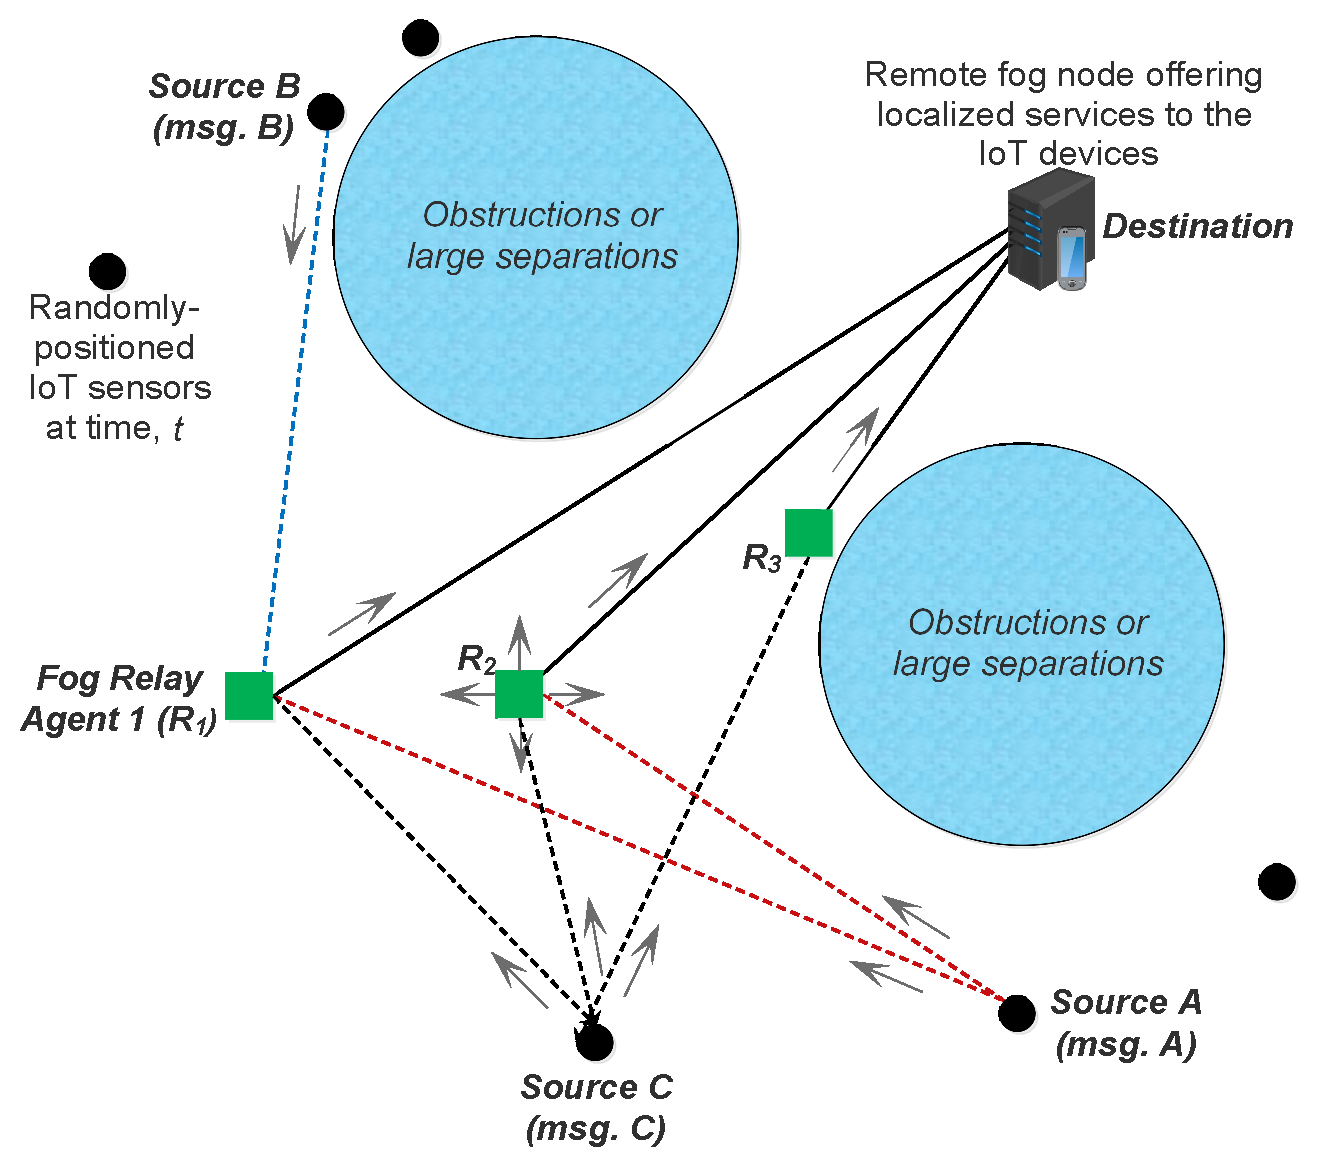
\includegraphics[width=3.2in]{ideafig1.eps}
 %where an .eps filename suffix will be assumed under latex,
% and a .pdf suffix will be assumed for pdflatex; or what has been declared
% via \DeclareGraphicsExtensions.
\caption{Single-agent fog-based IoT system.}
\label{ideafig1}
\end{figure}

\section{Problem Definition}
In this section, we provide full description of the system model, as well the RL approach used to address the problem. The Mobile Fog Relay Agent (MFRA) and its environment are discussed below.

\subsection{MFRA environment}
\emph{\textbf{States}}: The states are defined as a tuple, $\langle$Outage communication cost ($\mathcal{P}_{out}$) /Energy status of the fog relay (J) /Energy status of the IoT sensor (J)$\rangle$.

\begin{itemize}
  \item Outage communication cost: Outage observations from the environment is estimated using (\ref{eqn1a}) from \cite{OmoniwaRelay2018}, which gives an estimate of the communication outage when the agent takes an action, such as changing power levels or location, or both.
  \item Energy expended by fog relay: This observation gives the agent insight on how much energy by the fog agent when following policy~$\omega_i \in \omega_{fog}$. If the fog agent continues to take sub-optimal actions, it depletes its energy and dies out.
  \item Energy expended by IoT sensor: This observation gives the agent insight on how much energy the IoT sensor has used up by following a policy~$\omega_i \in \omega_{IoT}$. If the IoT sensor continues to take sub-optimal actions, it depletes its energy and dies out.
\end{itemize}


\begin{equation}\label{eqn1a}
  \mathcal{P}_{out} = 1 - (1 + 2\Psi^2 \ln \Psi) \exp\Big( -\frac{N_0 \tilde{\kappa}}{P_{I} (D_{I} + \delta)^{-\sigma}}\Big),
\end{equation}


where~$\Psi = \sqrt{(N_0 \tilde{\kappa})/(P_{R}(D_{S} + \delta)^{-\sigma})}$, and~$\mathcal{P}_{out}$ is an expression for the outage probability with values between 0 and 1. We assume a predefined threshold~$\tilde{\kappa}$ which determines the outage in communication,~$P_{I}$ is transmit power of the IoT sensor,~$P_{R}$ is transmit power of the fog relay agent,~$D_{I}$ is the distance between IoT sensor and fog relay agent, and~$D_{S}$ is the distance between fog relay agent and destination node. We assume a small change in the position of the fog relay agent,~$\delta = \pm0.25 m$,~$N_0$ to be the channel noise, and~$\sigma$ to be the path-loss exponent.



\subsection{MRFA agent}
We apply a the Q-Learning algorithm, an RL approach which requires no prior knowledge of the environment by the agent. In Q-learning, the agent interacts with the environment over periods of time according to a policy~$\omega$. At every time-step~$k \in N$, the environment produces an observation~$s_{k} \in \mathbb{R}^{D_s}$. By sampling, the agent then picks an action~$a_{k}$ over~$\omega(s_{k})$,~$a_{k} \in \mathbb{R}^{D_a}$, which is applied to the environment. The environment consequently produces a reward~$r(s_{k}, a_{k})$ and may end the episode at state~$s_{N}$ or transits to a new state~$s_{k + 1}$. The agent's goal is to minimize the expected cumulative cost,~$\min_{\omega} \mathbb{E}_{s_0, a_0, s_1, a_1, ..., s_N} \Big[ \sum_{i=0}^{N} \gamma^i \mathcal{C}(s_i) \Big]$, where~$0 \leq \gamma \leq 1$ is the discount factor, and~$\mathcal{C}$ is the overall cost function of our model.

First, the agent takes an initial random action~$a_{k}$ and gets observations from the environment which corresponds to that action, as well as a reward. It then discretizes the continuous observations emanating from the environment into a~$50 \times 5 \times 5$ state space corresponding to the tuple, $\langle$Outage communication cost ($\mathcal{P}_{out}$) /Energy status of the fog relay (J) /Energy status of the IoT sensor (J)$\rangle$. The agent then updates it's Q-values at each time-step~$k$ following (\ref{eqn1b}).

\begin{equation}\label{eqn1b}
\begin{split}
Q(s_k, a_k) &:= Q(s_k, a_k)\\
& + \alpha \Big[ r_{k + 1} + \gamma \max_{a}  Q(s_{k + 1}, a) -  Q(s_k, a_k) \Big],
   \end{split}
\end{equation}
where~$\alpha$ is the learning rate, which determines the impact of new experience on the Q-value,~$r_{k + 1}$ is the reward the agent receives by being in~$s_{k + 1}$ from~$s_{k}$. Based on the policy followed by the agent, it gets observations and rewards from the environment.

\emph{\textbf{Action space}}: The actions are move and transmit by fog relay, and select a power-level and transmit by IoT end-device, which make up eight possible actions.

 \begin{itemize}
  \item Mobility: Move by $\pm \delta$ and transmit, where~$\delta = \pm0.25m$ and mobility range (m) = [-30, 30]
  \item Power-level: Choose power-level and transmit, $P$, where~transmit power ranges (W) = [0.001, 0.01, 0.15, 0.2, 0.25, 0.3]
\end{itemize}

\emph{\textbf{Goal}}: The goal is for the agent to learn to minimize the overall cost~$\mathcal{C}$ in the tuple, $\langle$Outage communication cost ($\mathcal{P}_{out}$) /Energy status of the fog relay (J) /Energy status of the IoT sensor (J)$\rangle$, by keeping all nodes within the link alive while ensuring that the packets received in each transmission does not fall below the pre-defined threshold, which was set at 95\%.

\emph{\textbf{Rewards}}: The reward function used is given in (\ref{eqn1c}) as

 \begin{equation}\label{eqn1c}
    R =
    \begin{cases}
      100, & \text{if}\ goal==Reached \\
      0, & \text{otherwise.}
    \end{cases}
  \end{equation}


\emph{\textbf{Metrics}}: Outage probability, i.e. the ratio of the number of packet lost to those transmitted, which we measure in percentages, and energy status of the fog relay agent and the IoT sensor, i.e. the ratio of depleted energy to the initial capacity in Joules, which we measure as a percentage.


The MFRA's learning process is summarized in Algorithm \ref{fiotRL}. A new learning episode is terminated when the agent attains the pre-defined goal of minimizing the communication outage in the link, or when either the fog relay or the IoT sensor dies out due to taking sub-optimal actions without getting to the goal. When an fog relay moves closer to the communicating parties, the IoT sensor uses a lower power level as compared to when it is far away, hereby saving IoT sensor energy. However, mobility have some cost and if the fog relay continues to move in order to minimize the communication outage, it may die out soon, hereby causing a point-of-failure to the network. As each episode is completed, a reward of 100 points is given to the agent if it reaches its goal and a 0 points otherwise. The reward is updated in the Q-learning table, with environmental information updated as well.

\begin{algorithm}
\caption{MFRA Learning Process}\label{fiotRL}
\begin{algorithmic}[1]
\State \textbf{Initialize:} Power levels (W) = [0.001, 0.01, 0.15, 0.2, 0.25, 0.3],~$\delta = \pm0.25m$ and mobility range (m) = [-30, 30]
\BState \emph{top}:
\State ResetEnvironment()
\State \emph{state} $\leftarrow$ MapLocalObservationToState(\emph{env})
\State \emph{action} $\leftarrow$ QLearning.SelectAction(\emph{state})
%\BState \emph{top}:
\If { \emph{action}  == ``move close and Tx''} %\Return stop,
\State Env.EstimateOutage (\ref{eqn1a})
\State Env.EstimateFogEnergyStatus
\ElsIf {\emph{action}  == ``move away and Tx''}
\State Env.EstimateOutage (\ref{eqn1a})
\State Env.EstimateSensorEnergyStatus
\ElsIf { \emph{action}  == ``choose power level and Tx''}
\State Env.EstimateOutage (\ref{eqn1a})
\State Env.EstimateSensorEnergyStatus
\EndIf
\State \textbf{endif}
\State InvokePolicy(ExponentialDecay)
\State UpdateQLearningProcedure() (\ref{eqn1b})
\State CurrentState $\leftarrow$ NewState
\If { \emph{goal}  == ``Reached''}  \Return Reward = 100,
\ElsIf { \emph{goal}  != ``Reached'' or Agent == Death}  \Return Reward = 0
\EndIf
\State \textbf{endif}
\State EndEpisode \textbf{goto} \emph{top}.
\end{algorithmic}
\end{algorithm}



\section{Experimental Setup}
We carried out experimentation using the Python IDE 3.7.2, and considered a single agent to help us compare our proposed approach with the baseline.

\subsection{Baselines}
The baseline~\cite{OmoniwaRelay2018} used for the comparative analysis applied a gradient descent approach to arrive at a local optima in minimizing the communication outage within the network. The baseline approach is known to arrive at a local optima, however, may take significant amount of time to converge.

\subsection{Indicators}
To evaluate our proposed approach, we examine the convergence of our approach in minimizing the steps it takes the agent to get to its goal, the energy utilization of the fog relay and IoT sensor.



\section{Results and Discussions}
In this section, we present the results of the fog-based IoT system. First, we compare the proposed approach with the baseline, then we examine the number of steps required by the agent to reach it's goal over learning episodes. Finally, we evaluate the energy utilization of both the fog relay agent and the IoT sensor.

\subsection{Proposed approach vs. baselines}
We carried out comparison of the proposed approach, applying the Q-learning algorithm and the baseline, using the gradient descent algorithm. Simulations were done using Python IDE 3.7.2, and Table~\ref{table:simparameters} shows a summary of the parameters used. Fig. \ref{pckt_sent} shows the percentage of packets successfully transmitted, with each algorithm learning to minimize the number of packets lost over each episode. We observe that in the first 20 episode, the baseline had better performance than the proposed approach, however, for the remaining part of the episodes, the proposed approach out-performed the baseline. This signifies that the agent's exploration within the environment plays some significant role in improving the packets successfully transmitted. Convergence can be observed around 200th episodes where about 55\% - 100\% of transmitted packets are successfully received at the destination. Interestingly, we know that gradient descent methods may be slow to converge, but always surely converge to a local optima~\cite{OmoniwaRelay2018}. This is well depicted Fig. \ref{pckt_sent}, where around 1000th episode the baseline approach is able to successfully transmit about 75\% of packets.

\begin{table}
\small
\centering
\caption{Simulation Parameters}
\label{table:simparameters}
\begin{tabular}{ll}
  \hline
 \textit{Parameter} & \textit{Values} \\
  \hline \hline

   $D_{I}$ & 40 metres\\
   $P_{I}$ & [0.001, 0.3] Watts \\
   $D_{S}$ & 35 metres\\
   $P_{R}$ & 0.3 Watts\\
   $\delta$ & $\pm0.25$ metres\\
   Mobility bound & [-35,~35] metres\\
   Noise power $N_0$ & $2 \times 10^{-7}$ Watts\\
   Path-loss exponent $\sigma$ & 3\\
   Pre-defined threshold $\kappa$ & 1\\
   Discount factor $\gamma$ & 0.9\\
   Learning rate $\alpha$ & 0.1\\
   Episodes $N$ & 1000\\
   Iteration runs & 100000\\
   Policy $\epsilon$ & $e^{-0.0015N}$\\

   \hline \hline
 \end{tabular}
 \end{table}

\begin{figure}[!t]
\centering
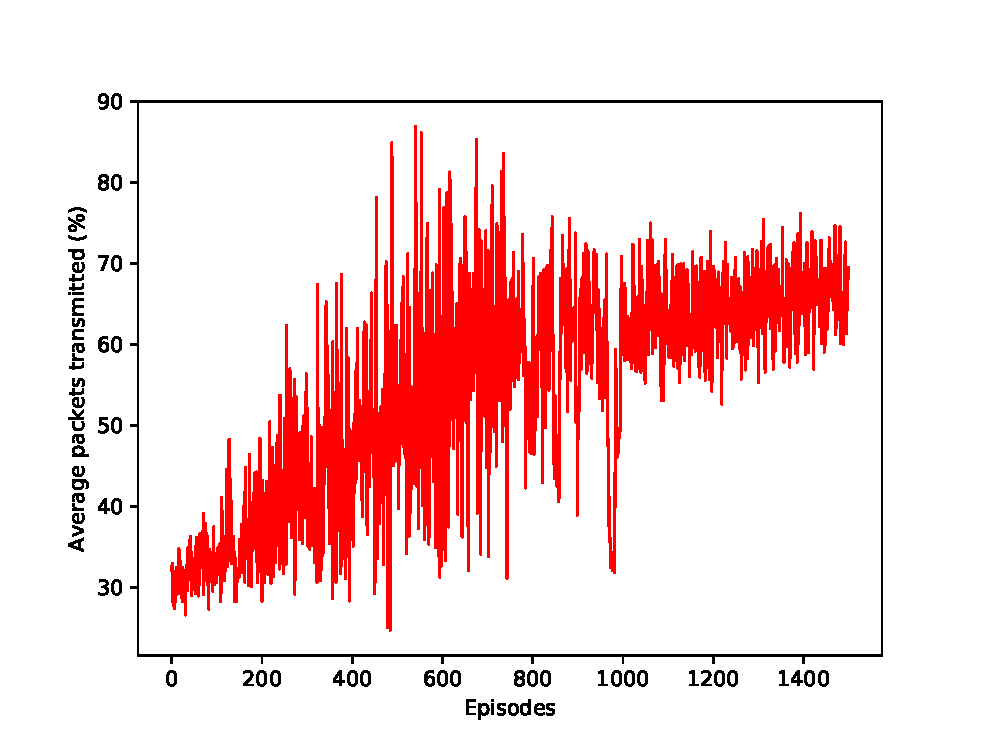
\includegraphics[width=3.8in]{pckt_sent.eps}
 %where an .eps filename suffix will be assumed under latex,
% and a .pdf suffix will be assumed for pdflatex; or what has been declared
% via \DeclareGraphicsExtensions.
\caption{Percentage of packets successfully transmitted.}
\label{pckt_sent}
\end{figure}

Overall, the performance of the proposed approach yields better results than the baseline. In Fig. \ref{num_iter}, we observe the number of iterations required for the agent to reach it's goal following policy~$\epsilon$. After 200 episodes, we achieve convergence. This implies that the agent learns to reach the goal state faster and more efficiently. Similarly, in Fig. \ref{rew_iter}, which shows the number of iterations per reward, convergence was attained at about 200 episodes. This implies that the agent learns to follow policies that maximize its total expected reward. Therefore, the proposed RL approach has shown good performance behaviour as compared to the previous approach.


\begin{figure}[!t]
\centering
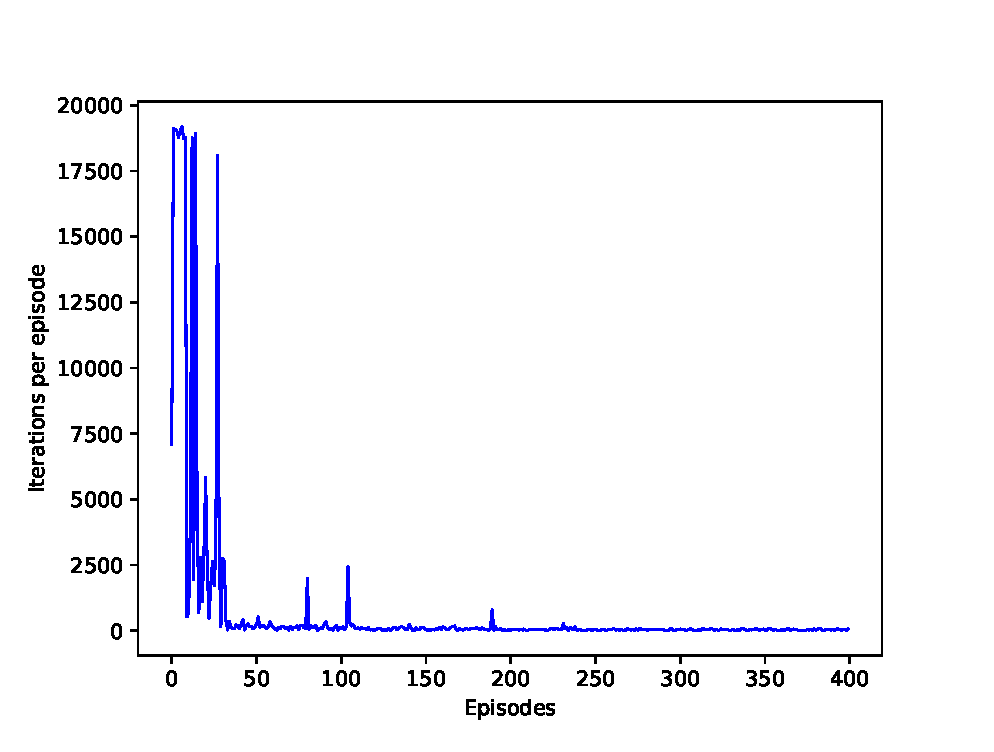
\includegraphics[width=3.8in]{num_iter.eps}
 %where an .eps filename suffix will be assumed under latex,
% and a .pdf suffix will be assumed for pdflatex; or what has been declared
% via \DeclareGraphicsExtensions.
\caption{Number of iteration over episodes.}
\label{num_iter}
\end{figure}


\begin{figure}[!t]
\centering
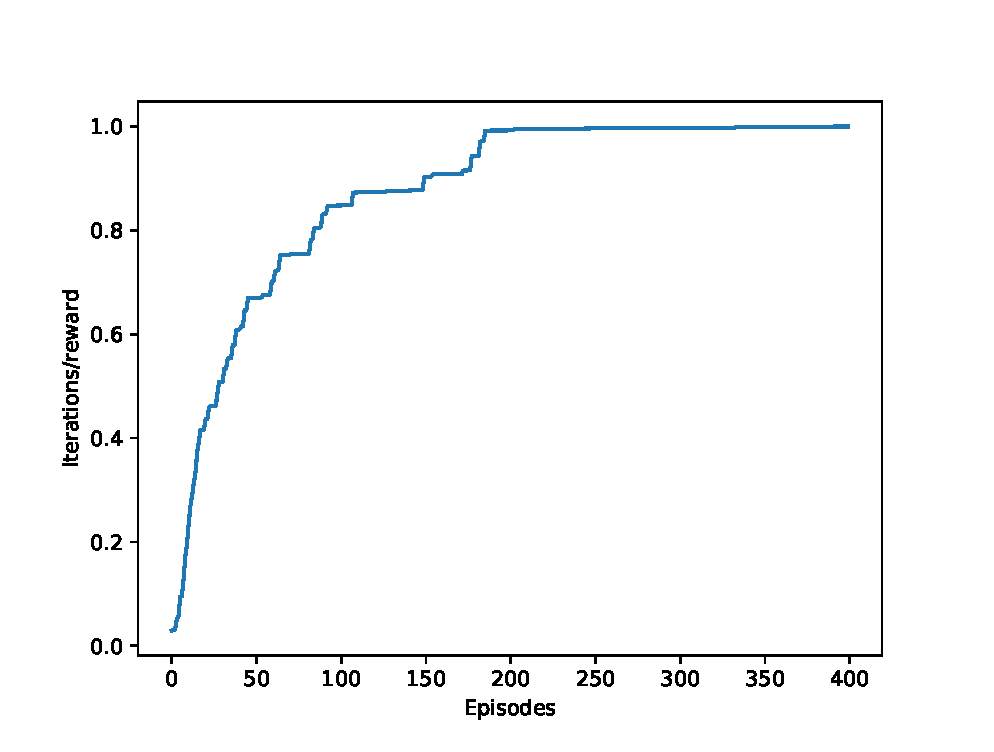
\includegraphics[width=3.8in]{rew_iter.eps}
 %where an .eps filename suffix will be assumed under latex,
% and a .pdf suffix will be assumed for pdflatex; or what has been declared
% via \DeclareGraphicsExtensions.
\caption{Normalized Iterations per reward over 1000 episodes.}
\label{rew_iter}
\end{figure}

\subsection{Energy utilization}
We examine the impact of the learning process on the energy utilization of both the fog relay and the IoT sensor. Fig. \ref{energy_fog}, shows the energy consumed by the fog relay during transmission. We observe that at about 50 episodes, the fog relay consumes less than 10\% of its energy in moving and transmitting. This has significant impact to increasing the longevity of fog devices within the network. A similar behaviour is also observed for the IoT sensor shown in Fig. \ref{energy_iot}, where the IoT sensor after about 60 episodes, spends less than 10\% of its energy on transmission. The outcome of this experiments reveal that energy management within the IoT domain can be efficiently tackled using RL approach.


\begin{figure}[!t]
\centering
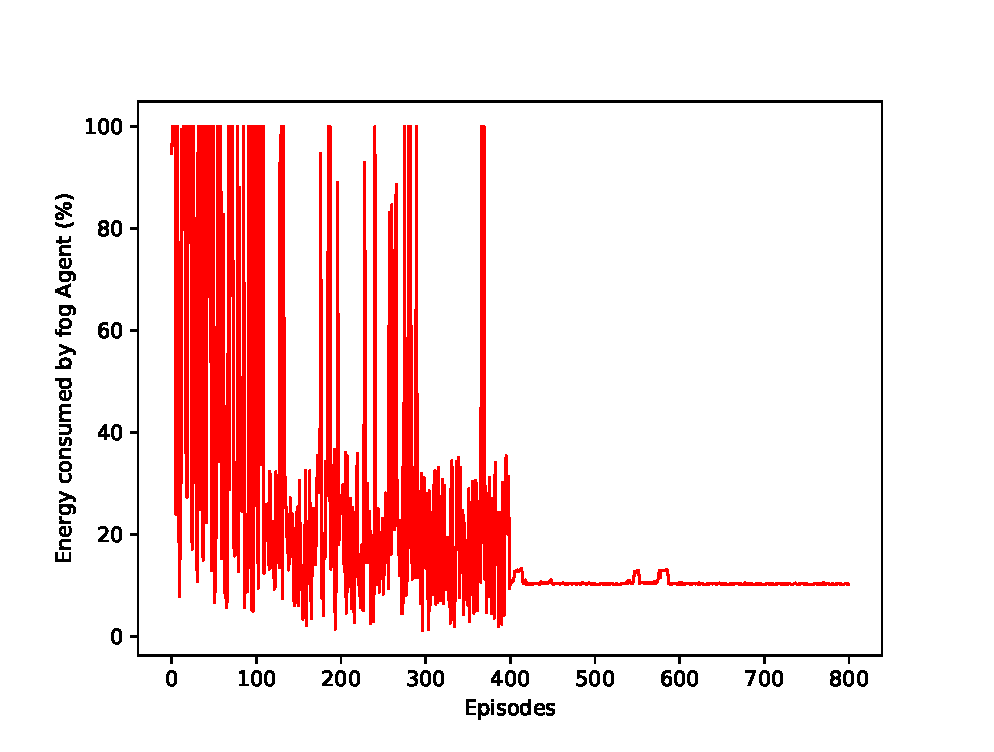
\includegraphics[width=3.8in]{energy_fog.eps}
 %where an .eps filename suffix will be assumed under latex,
% and a .pdf suffix will be assumed for pdflatex; or what has been declared
% via \DeclareGraphicsExtensions.
\caption{Energy consumed by fog agent over episodes.}
\label{energy_fog}
\end{figure}

\begin{figure}[!t]
\centering
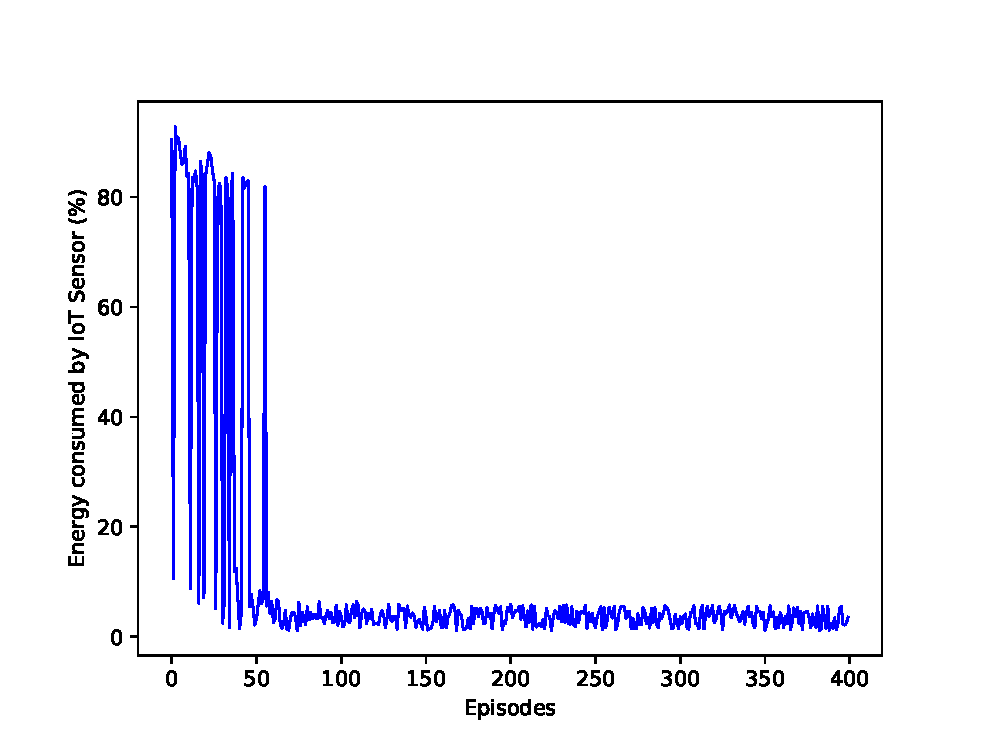
\includegraphics[width=3.8in]{energy_iot.eps}
 %where an .eps filename suffix will be assumed under latex,
% and a .pdf suffix will be assumed for pdflatex; or what has been declared
% via \DeclareGraphicsExtensions.
\caption{Energy consumed by IoT sensor over episodes.}
\label{energy_iot}
\end{figure}




\section{Related Works}
Considering the dynamics and heterogeneity within the ultra-distributed IoT environment, it is important for communication devices which are mobile to move seamlessly without degrading quality of service (QoS). More so, the constrained devices should communicate efficiently without depleting all their energy by transmitting at high-power, which may have long-term consequences to the network. Several non-RL-based approaches have been proposed to optimize the communication performance in IoT based networks, however, when some parameters in the network are changed, these approaches may fail.
The work in~\cite{OmoniwaRelay2018} considered a multi-tier fog-based IoT architecture where a mobile/static fog node acts as an amplify and forward relay that transmits received information from a IoT sensor node to a higher hierarchically-placed fog device, which offers some localized services. In order to minimize the outage in communication, an iterative algorithm based on the steepest descent method (SDM) was proposed to jointly optimize the mobility pattern and power-control parameters. However, the single-agent based work did not take into consideration the performance of the approach in a highly-decentralised IoT environment. Furthermore, each time the topology is changed, the agent will need to recompute the model in other to act optimally.

RL can be applied to a new environment, since the it allows the agent to learn, by take actions that will improve its long-term return. Furthermore, RL can be applied to multiple agents. In \cite{Wilhelmi2017}, a decentralised, multi-agent-based stateless Q-learning approach was proposed, where no information about neighbouring nodes are available to agents. Though the paper was able to improve aggregate throughput in the network, by allowing the networks modify both the transmission power and the channel used, however, high variability was observed in the throughput of the individual networks. Only eight agents were observed using a stateless Q-learning approach. The work did not adequately depict the distributed nature of the IoT network. Moreover, mobility of agents was completely ignored.

Several works in WSN have applied the decentralised RL technique. In \cite{Liang2009}, a multi-agent reinforcement learning-based multi-hop mesh cooperative (MRL-CC) mechanism for the improvement of some QoS metrics in the WSNs. Though the mobility of the cooperative nodes were taken into account when learning the optimal policy, the MRL-CC failed to consider the power dissipated by the power-constrained devices, as well as the overall outage in communication.

In \cite{Chen2008}, a reliable and energy-efficient routing (REER) protocol was proposed using a geographic routing approach. The work considered the idea of a central entity, called a reference node (RN), which is assumed to be situated at an ideal location between source and destination. Several other cooperative nodes, which contend to relay data, are assumed to be situated around the RN. The work was able to examine the trade-off between reliability and energy-efficiency when the distances between RNs was adjusted.


We present a decentralised reinforcement learning approach that adequately addresses some key performance issues within the IoT domain.
The main task of our work is to minimize global outage in communication within a fog-based IoT network, by optimizing the power-control parameter of the potential mobile fog-relay agent (MFRA), as well as optimizing the position of each relaying agents in the network. As such, each MFRA is compelled to take certain actions that may influence its environment. However, the duration it takes the MFRA to learn is significantly influenced by the state space, as well as the possible set of actions~\cite{Dusparic2009}. The variables for the state, action and reward of an agent may be discrete or continuous, with the former represented as small interval of values which imply distinct levels~\cite{Yau2012}, and can easily be represented in a tabular form. However, it is difficult to represent continuous space using Q-learning tables. The work in \cite{Vucevic2007} considered a RL agent that explores continuous state and action space using Gaussian unit search behaviour. Other works~\cite{Dusparic2009, Cuayahuitl2006} considered the reduction of states by eliminating states that are unlikely to occur. However, this may pose a big risk especially in a highly dynamic environment. RL can be effective for learning action policies in discrete stochastic environments, but its efficiency can decay exponentially with increasing state space~\cite{Uther1998}. Our proposed problem can be observed to have continuous state-action pairs, and is approached by discretizing the state and action space.


In this paper, we assume the following.
\begin{enumerate}
  \item The MFRA is completely oblivious of its environment, and as such, has no prior knowledge of the overall cost function.
  \item The MRFA may change its position in order to ensure better communication. Also, the MFRA may change its position (2D/3D) depending on the scenario considered.
  \item The MFRA has an objective of learning to make actions that yield better outcomes within its local view of the environment.
  \item The states are be divided into discrete levels to overcome the exponential decay in the efficiency of the proposed approach due infinite state space.
  \item The MFRA independently tries to optimize power usage and moves in a direction that maximizes the communication outage.
\end{enumerate}





\section{Conclusion and Future works}
We aim to apply the q-learning algorithm on a multi-agent fog-based IoT system where multiple agents compete to transmit reliably in a highly dynamic environment, where interference contributes significantly to communication outages with the network. For instance, agents may take actions that can have direct consequences on neighbouring agents, which may have further impact on other agents within the network. For instance, if an agent decides to increase the transmit power beyond some threshold value, in order to boost its communication capabilities, its action may result in channel interference to its immediate neighbours, and worst, it may deplete its energy fast, and die-out, leading to link failure that can affect the performance of the entire network. This will be looked at in our future work.




\ifCLASSOPTIONcaptionsoff
  \newpage
\fi

%\newpage

% trigger a \newpage just before the given reference
% number - used to balance the columns on the last page
% adjust value as needed - may need to be readjusted if
% the document is modified later
%\IEEEtriggeratref{8}
% The "triggered" command can be changed if desired:
%\IEEEtriggercmd{\enlargethispage{-5in}}

% references section

% can use a bibliography generated by BibTeX as a .bbl file
% BibTeX documentation can be easily obtained at:
% http://mirror.ctan.org/biblio/bibtex/contrib/doc/
% The IEEEtran BibTeX style support page is at:
% http://www.michaelshell.org/tex/ieeetran/bibtex/
%\bibliographystyle{IEEEtran}
% argument is your BibTeX string definitions and bibliography database(s)
%\bibliography{IEEEabrv,../bib/paper}
%
% <OR> manually copy in the resultant .bbl file
% set second argument of \begin to the number of references
% (used to reserve space for the reference number labels box)
\begin{thebibliography}{1}
\bibitem{Omoniwa2018}
B. Omoniwa, R. Hussain, M. A. Javed, S. H. Bouk and S. A. Malik, "Fog/Edge Computing-based IoT (FECIoT): Architecture, Applications, and Research Issues," in IEEE Internet of Things Journal.

\bibitem{Chiangh2016}
M. Chiang and T. Zhang, ``Fog and IoT: An Overview of Research Opportuinities,'' IEEE Internet of Things, vol. 3, no. 6, pp. 854-864, Dec.
2016.

\bibitem{OmoniwaRelay2018}
B. Omoniwa et al., "An Optimal Relay Scheme for Outage Minimization in Fog-based Internet-of-Things (IoT) Networks," in IEEE Internet of Things Journal.

\bibitem{Wilhelmi2017}
F. Wilhelmi, B. Bellalta, C. Cano and A. Jonsson, "Implications of decentralized Q-learning resource allocation in wireless networks," 2017 IEEE 28th Annual International Symposium on Personal, Indoor, and Mobile Radio Communications (PIMRC), Montreal, QC, 2017, pp. 1-5.

\bibitem{Mozaffari2016}
M. Mozaffari, W. Saad, M. Bennis and M. Debbah, "Mobile Internet of Things: Can UAVs Provide an Energy-Efficient Mobile Architecture?," 2016 IEEE Global Communications Conference (GLOBECOM), Washington, DC, 2016, pp. 1-6.

\bibitem{Gueriau2018}
M. Gueriau and I. Dusparic, "SAMoD: Shared Autonomous Mobility-on-Demand using Decentralized Reinforcement Learning,"  1558-1563. 10.1109/ITSC.2018.8569608.

\bibitem{Azari2018}
A. Azari and C. Cavdar, "Self-organized low-power IoT networks: A distributed learning approach," arxiv


\bibitem{Dusparic2009}
I. Dusparic and V. Cahill, ``Distributed W-Learning: Multi-Policy Optimization in Self-Organizing Systems,'' 2009 Third IEEE International Conference on Self-Adaptive and Self-Organizing Systems, San Francisco, CA, 2009, pp. 20-29.


%%%%%%%%%%%%%WSN
\bibitem{Chen2008}
M. Chen, T. Kwon, S. Mao, Y. Yuan and V. C. M. Leung, ``Reliable and energy-efficient routing protocol in dense wireless sensor networks,'' Int. J. Sen. Netw.
 vol. 4, no. 1/2, pp. 104-117, July 2008.


\bibitem{Liang2009}
Xuedong Liang, Min Chen, Yang Xiao, I. Balasingham and V. C. M. Leung, ``A novel cooperative communication protocol for QoS provisioning in wireless sensor networks,'' 2009 5th International Conference on Testbeds and Research Infrastructures for the Development of Networks and Communities and Workshops, Washington, DC, 2009, pp. 1-6.

\bibitem{Yau2012}
K.-L. A. Yau, P. Komisarczuk, P. D. Teal, ``Reinforcement learning for context awareness and intelligence in wireless
networks: Review, new features and open issues,'' Journal of Network and Computer Applications, vol. 35, no. 1, pp. 253-267, Jan. 2012.

\bibitem{Vucevic2007}
N. Vucevic, J. Perez-Romero, O. Sallent and R. Agusti, "Reinforcement Learning for Active Queue Management in Mobile All-IP Networks," 2007 IEEE 18th International Symposium on Personal, Indoor and Mobile Radio Communications, Athens, 2007, pp. 1-5.

\bibitem{Uther1998}
W. T. B. Uther and M. M. Veloso, ``Tree Based Discretization for Continuous State Space Reinforcement Learning,'' \emph{Proceedings of the Fifteenth National/Tenth Conference on Artificial Intelligence/Innovative Applications of Artificial Intelligence,} 1998, Madison, Wisconsin, USA, pp. 769-774.

\bibitem{Cuayahuitl2006}
H. Cuayahuitl, S. Renals, O. Lemon, and H. Shimodaira. ``Learning multi-goal dialogue strategies using reinforcement learning with reduced state-action spaces,'' In Int. Journal of Game Theory, pp. 547–565, 2006.
\end{thebibliography}


% that's all folks
\end{document}


